\chapter{Vector Equations} \label{ch:3VectorEqns}
\tstk{non-crash citation \cite{graham2018citation}}
This file should include the work on vector-curl equations, and have a similar sort of feel to it as the scalar case. Indeed, it should even refer back to the previous section and draw the appropriate parallels.

\section{The Vector Sobolev Spaces} \label{sec:VectorSobSpaces}
\tstk{I guess some references here would be good too, like another Zhikov if it exists, plus Kirill \& Serena's paper.}
In chapter \ref{ch:2ScalarEqns} we introduced the concept of gradients with respect to arbitrary measures $\nu$ and their associated Sobolev spaces.
Here we proceed to define a similar notion for curls and vector-valued functions.
Let $D\subset\reals^3$, $\nu$ be a (Borel) measure on $D$, and let $W=W\bracs{D,\nu}$ be the closure of the set of pairs $\bracs{\phi, \grad\wedge\phi}$ in $\ltwo{D}{\nu}^3\times\ltwo{D}{\nu}^3$ for $\phi\in\smooth{D}$.
An element of $W$ is a pair $\bracs{u,z}$ and we agree to denote the component $z$ by $z=\curl{\nu}u$ and refer to it as a ``curl of $u$ with respect to $\nu$" although given the analysis of section \ref{sec:ScalarSobSpaces} it may be unsurprising to learn that this terminology requires some qualification.
The Sobolev space $\curlSob{D}{\nu}$ is then the collection of first components $u$,
\begin{align*}
	\curlSob{D}{\nu} &= \clbracs{u \ \vert \ \bracs{u,\curl{\nu}u}\in W}.
\end{align*}

One can quickly deduce that $\nu$-curls are not unique by employing a similar argument to the case of $\nu$-gradients; if both $\bracs{u,z}$ and $\bracs{0,y}$ are elements of $W$ then clearly $\bracs{u,y+z}\in W$ too.
\tstk{tangential curl argument! has this been done in full??? If not we need to be inspired by Zhikov!}
\tstk{also the density arguments, but these are needed anyway for the tang. curl args.}

\tstk{now onto differential equations involving curls.}

\section{Curls of Zero - a need for care}
The notion or interpretation of the curl is not as straightforward as that of the gradient, and this can lead to some unexpected results when we make the leap to curls with respect to non-Lebesgue measures.
We aim to illustrate one of these somewhat unexpected results, and then develop an intuitive understanding of the concept of the notion of curl defined in section \ref{sec:VectorSobSpaces}. \newline

Let $\dddom\subset\reals$ and let $I\subset\reals$ be an interval, so the segment $\widetilde{I} := I\times\clbracs{0}\times\clbracs{0}\subset\dddom$ is parallel to the $x_1$-axis.
Let $\lambda_I$ denote the measure on $\dddom$ that supports 1D-Lebesgue measure down the segment $\widetilde{I}$.
We wish to characterise the set $\curlZero{\dddom}{\lambda_I}$, by density we will only need to consider functions in $\smooth{\dddom}^3$. \newline

Let $u\in\smooth{\dddom}^3$, and set $v = \bracs{0,0,u}^{\top}$.
We can see that $v\in\curlZero{\dddom}{\lambda_I}$ because the smooth functions\footnote{Strictly speaking, we should consider this as a constant sequence of smooth functions.} $\phi = \bracs{-x_2 u, 0, 0}^{\top}$ satisfy
\begin{align*}
	\integral{\dddom}{\abs{\phi}^2}{\lambda_I} &= \integral{\dddom}{x_2^2\abs{u}^2}{\lambda_I} \\
	&= 0 \text{ as } x_2=0 \text{ on } \widetilde{I}.
\end{align*}
By computation, $\grad\wedge\phi = \bracs{0, -x_2\partial_3 u, u}^{\top}$ and so we also find that
\begin{align*}
	\integral{\dddom}{\abs{\grad\wedge\phi - v}^2}{\lambda_I}
	&= \integral{\dddom}{0 + \abs{-x_2\partial_3 u}^2 + \abs{u-u}^2}{\lambda_I} \\
	&= \integral{\dddom}{x_2^2\abs{\partial_3 u}^2}{\lambda_I} \\
	&= 0.
\end{align*}
Thus we conclude that $v\in\curlZero{\dddom}{\lambda_I}$.
One obtains a similar result when considering $v=\bracs{0, u, 0}^{\top}$ and using the function $\phi = \bracs{x_3 u, 0 , 0}^{\top}$.
Thus we have established (after density arguments) that
\begin{align*}
	 \mathrm{span}\clbracs{
	 \begin{pmatrix} 0 \\ u \\ 0 \end{pmatrix}, \begin{pmatrix} 0 \\ 0 \\ u \end{pmatrix}
	 \ \vert \ u\in\ltwo{\dddom}{\lambda_I}
	 }\subset \curlZero{\dddom}{\lambda_I}
\end{align*}
So far this is unsurprising if think back to the gradient case in section \ref{sec:ScalarSobSpaces} - the measure $\lambda_I$ only ``sees" along $\widetilde{I}$ and the two examples we have considered thus far are both directed ``out of" $\widetilde{I}$.
However we can also show that any $v=\bracs{u,0,0}^{\top}\in\curlZero{\dddom}{\lambda_I}$ too (for $u\in\smooth{\dddom}$), by exploiting the function $\phi=\bracs{0,-x_3 u,0}^\top$.
Thus we are forced to conclude that $\curlZero{\dddom}{\lambda_I} = \ltwo{\dddom}{\lambda_I}^3$, that is that every function is a curl of zero! \newline

This result is quite perplexing at first, however a similar example can help us shed some light onto the matter.
We now consider a plate $P = \clbracs{0}\times I_2\times I_3$ in $\dddom\subset\reals^3$, and let $\dddmes$ be the measure that supports 2D Lebesgue measure on the plate $P$.
Looking to characterise $\curlZero{\dddom}{\dddmes}$ we quickly establish that
\begin{align*}
	\begin{pmatrix} 0 \\ u \\ 0 \end{pmatrix}, \begin{pmatrix} 0 \\ 0 \\ u \end{pmatrix}
	\in \curlZero{\dddom}{\dddmes} \quad \forall u\in\smooth{\dddom},
\end{align*}
by considering the functions $\phi=\bracs{0, 0, -x_1 u}$ and $\phi=\bracs{0, x_1 u, 0}$ and using the fact that $x_1=0$ on $P$.
After density arguments, this tells us that
\begin{align*}
	 \mathrm{span}\clbracs{
	 \begin{pmatrix} 0 \\ u \\ 0 \end{pmatrix}, \begin{pmatrix} 0 \\ 0 \\ u \end{pmatrix}
	 \ \vert \ u\in\ltwo{\dddom}{\dddmes}
	 }\subset \curlZero{\dddom}{\dddmes}
\end{align*}
We now verify that the only function of the form $v=\bracs{u,0,0}^\top$ that is an element of $\curlZero{\dddom}{\dddmes}$ is the zero function. \tstk{fill in these steps too}.

These two examples can be used to propose a notion of curl with respect to arbitrary measure.
One interprets the familiar classical curl of a function $u$ (that is, curl with respect to Lebesgue measure in 3D) as the axis of rotation of an infinitesimally small sphere placed within the vector field $u$.
The question we should be asking is ``how much of this rotation does the measure we are using actually see"?
Consider the plate example first, and the diagram drawn in figure \ref{fig:CurlInterpFigure}.
\begin{figure}[ht]
	\centering
	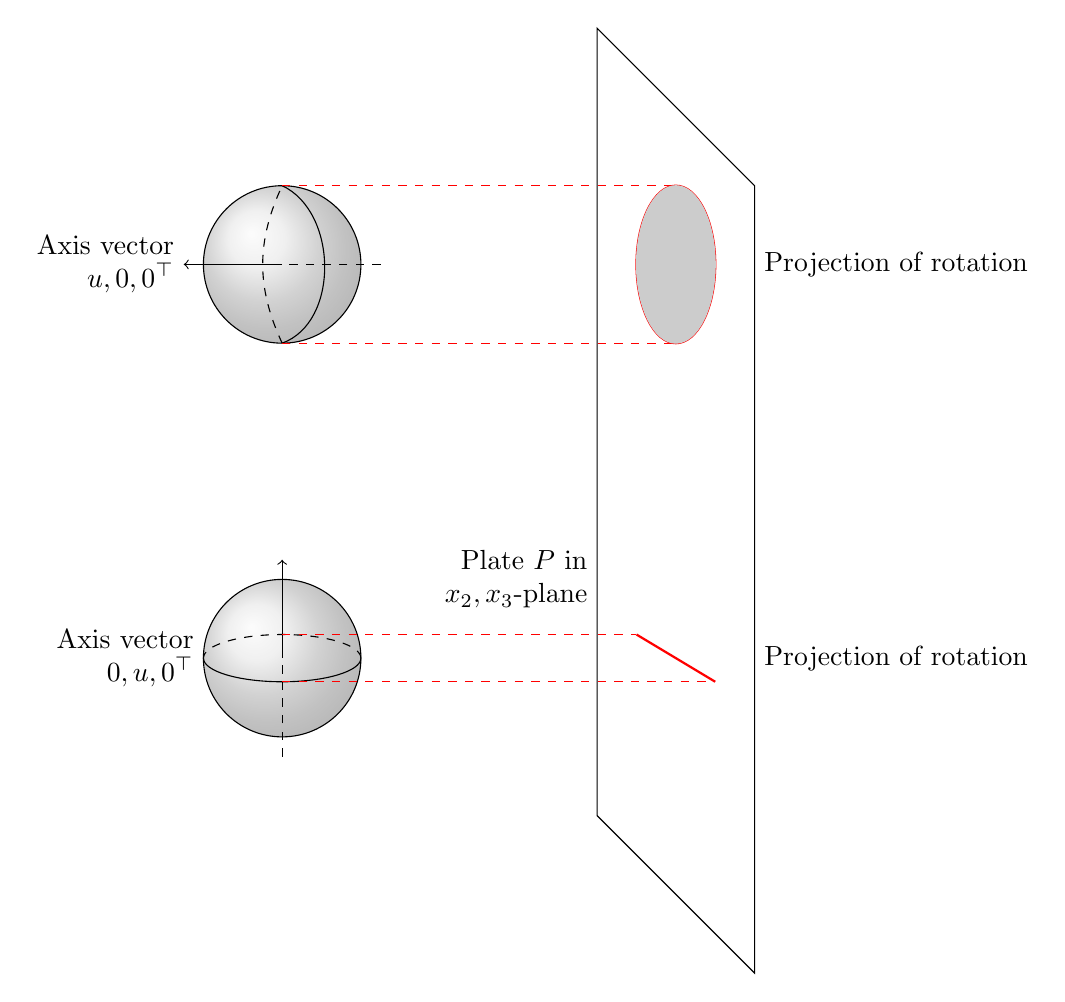
\begin{tikzpicture}
		%draw the plate itself as a parallelogram to induce a 3D effect
		\begin{scope}[shift={(4,0)}]
			\draw (0,0) -- (2,-2) -- (2,8) -- (0,10) -- cycle;
		\end{scope}
		
		%the ``infinitesimally small" sphere tilted on it's axis, perpendicular to the plane
		\begin{scope}[shift={(0,7)}, scale=0.5]
		  	\shade[ball color = gray!40, opacity = 0.4] (0,0) circle (2cm);
  			\draw (0,0) circle (2cm);
			\draw (0,-2) to[in=335, out=20] (0,2);
			\draw[dashed] (0,-2) to[in=245, out=115] (0,2);
  			%axis of rotation (perp to plane)
  			\draw[dashed] (2.5,0) -- (0,0);
  			\draw[->] (0,0) -- (-2.5,0);
		\end{scope}
		%now draw it's projection onto the plane...
		\begin{scope}[shift={(0,7)}]
			\draw[red, dashed] (0,1) -- (5,1);
			\draw[red, dashed] (0,-1) -- (5,-1);
%			\draw (5,-1) to[in=290, out=65] (5,1) to[in=205, out=115] cycle;
			\begin{scope}[xscale=0.5]
				\draw[red, thick] (2*5,0) circle (1cm);
				\filldraw[black!20!white] (2*5,0) circle (1cm);
			\end{scope}
		\end{scope}		
		
		%another ``infinitesimally small" sphere tilted on it's axis - this one is parallel to the plane (vert)
		\begin{scope}[shift={(0,2)}, scale=0.5]
		  	\shade[ball color = gray!40, opacity = 0.4] (0,0) circle (2cm);
  			\draw (0,0) circle (2cm);
  			\draw (-2,0) arc (180:360:2 and 0.6);
  			\draw[dashed] (2,0) arc (0:180:2 and 0.6);
  			%axis of rotation (|| to plane)
  			\draw[dashed] (0,-2.5) -- (0,0);
  			\draw[->] (0,0) -- (0,2.5);
		\end{scope}
		%now draw it's projection onto the plane...
		\begin{scope}[shift={(0,2)}]
			\draw[red, dashed] (0,0.3) -- (4.5,0.3);
			\draw[red, dashed] (0,-0.3) -- (5.5,-0.3);
			\draw[red, thick] (4.5,0.3) -- (5.5,-0.3);
		\end{scope}
		
		%some labels to be placed after we've moved and rescaled everything
		\node[anchor=east, align=right] at (4,3) {Plate $P$ in \\ $\bracs{x_2,x_3}$-plane};
		\node[anchor=east, align=right] at (-1,2) {Axis vector \\ $\bracs{0,u,0}^\top$};
		\node[anchor=east, align=right] at (-1.25,7) {Axis vector \\ $\bracs{u,0,0}^\top$};
		\node[anchor=west, align=left] at (6,7) {Projection of rotation};
		\node[anchor=west, align=left] at (6,2) {Projection of rotation};
	\end{tikzpicture}
	\caption{\label{fig:CurlInterpFigure} Diagram to illustrate the interpretation of curls of $\dddmes$. See the main body of text for the full explanation.}
\end{figure}
Consider the path traced out by a point on the surface of a sphere (of small radius) placed inside the vector field $u$, and the projection of this area onto the plate $P$. 
When the axis of rotation is perpendicular to $P$, this projection is a 2D subset of $P$ and has non-zero $\dddmes$-measure. 
If the axis is parallel to $P$, the projection is a 1D subset of $P$ and so has zero $\dddmes$-measure.
As such for a general axis of rotation $v$, the measure $\dddmes$ is only able to ``see" the rotation induced by the component of $v$ perpendicular to the plate $P$.
Now consider the same picture as in figure \ref{fig:CurlInterpFigure} but replacing the plate $P$ with a line segment $\widetilde{I}$.
In this case the projection of the area onto $\widetilde{I}$ is a finite set of at most two points, so will have zero $\lambda_I$-measure regardless of the axis of rotation $v$.
Hence our earlier conclusion that $\curlZero{\dddom}{\lambda_I}=\ltwo{\dddom}{\lambda_I}^3$, the measure $\lambda_I$ simply can't ``see" any rotation ``in $\widetilde{I}$".

\section{A Waveguide Problem}
The $k$-curls stuff and getting to the edge equations.
\tstk{about taking the Fourier transform, so now we're in 2D with a param $k$, and then refer back to section \ref{sec:ScalarExample} for the notation for the graph etc. Commented out stuff below might be useful for recycling this code.}
%As such we let $\dddom=\ddom\times I\subset\reals^2\times\reals$, where $\ddom$ will be the domain for our cross-sectional structure.
%We consider the plate $P=\mathset{0}\times I_2 \times I\subset\dddom$ and the singular measure $\dddmes$ that supports 2D Lebesgue measure on $P$.
%By assumptions on the waveguide geometry we can write $\dddmes=\ddmes \otimes \lambda_1$; and we would be looking to study the problem
%\begin{align} \label{eq:CurlProblemPreFT}
%	\curl{\dddmes}\bracs{\curl{\dddmes}u} &= \omega^2 u, \quad u\in\curlSob{\dddom}{\dddmes}
%\end{align}
%understood in the weak sense on $\dddom$.
%We take the Fourier transform in the $x_3$ direction, providing us with a family of problems in 2D obtains by transforming \eqref{eq:CurlProblemPreFT} and integrating out the $x_3$ dependence.
%The Fourier variable is denoted by $k\in\reals$, and we obtain for each $k$ the problem
%\begin{align} \label{eq:CurlProblem}
%	\curl{k}\bracs{\curl{k}u} &= \omega^2 u, \quad u\in\curlkSob{\ddom}{\ddmes}
%\end{align}
%where the operator $\curl{k}=\bracs{\partial_1,\partial_2,ik}^{\top}$ formally, and is understood with respect to the measure $\ddmes$.
%The space $\curlkSob{\ddom}{\ddmes}$ is the space we end up in after taking the Fourier transform, for a given $k$ it consists of $\ltwo{\ddom}{\ddmes}$ functions and their $k$-curls.
%As such we are now dealing with a 2D-problem with a measure $\ddmes$ that supports 1D Lebesgue measure down the segment $I_2\subset\ddom$.
%We seek to characterise the $k$-curls of zero and then derive the edge equations for \eqref{eq:CurlProblem}.

\subsection{The set $\kcurlZero{\ddom}{\ddmes}$} 
\tstk{need to do the full analysis, RN this is just for a single segment and then stops!}
We denote by $\kcurlZero{\ddom}{\ddmes}$ the set of all $k$-curls of the function $u\in\ltwo{\ddom}{\ddmes}$.
As when we were considering scalar-valued functions (see section \ref{sec:ScalarExample}), our interest here is in characterising the set of $k$-curls of zero. \newline

\subsubsection{Single Segments in the Plane}
We begin our analysis by considering the case when $\ddmes$ supports 1D Lebesgue measure along some segment $\clbracs{0}\times I_2\subset\ddom$, so $\ddmes=\lambda_{I_2}$.
With the goal of characterising $\kcurlZero{\ddom}{\lambda_{I_2}}$, consider some scalar $u\in\smooth{\ddom}$ and let $v = \bracs{0,u,0}^{\top}$ (again we only consider smooth $u$ because we can apply density arguments to extend the result to $\ltwo{\ddom}{\lambda_{I_2}}$ functions).
Now we observe that $v\in\kcurlZero{\ddom}{\lambda_{I_2}}$ because the (smooth) constant sequence $\phi^{(n)} = \phi = \bracs{0,0,-x_1 u}^{\top}$ satisfies;
\begin{align*}
	\integral{\ddom}{\abs{\phi}^2}{\lambda_{I_2}} &= \integral{I_2}{x_1^2\abs{u}^2}{\lambda_{I_2}} \\
	&= 0 \quad\text{as } x_1 = 0 \text{ on } I_2,
\end{align*}
and additionally
\begin{align*}
	\integral{\ddom}{\abs{\kcurl{\lambda_{I_2}}\phi - v}^2}{\lambda_{I_2}} &= \integral{\ddom}{\abs{\partial_2\phi_3 - ik\phi_2}^2}{\lambda_{I_2}} \\
	&+ \integral{\ddom}{\abs{ik\phi_1 - \partial_1\phi_3 - u}^2}{\lambda_{I_2}} + \integral{\ddom}{\abs{\partial_1\phi_2 - \partial_2\phi_1}^2}{\lambda_{I_2}} \\
	&= \integral{I_2}{x_1^2\abs{\partial_2 u}^2 + x_1^2\abs{\partial_1 u}^2}{\lambda_{I_2}} \\
	&= 0.
\end{align*}
Hence we have that
\begin{align} \label{eq:Curl0SeqConv}
	\phi^{(n)} \lconv{\ltwo{\ddom}{\lambda_{I_2}}^3},
	&\quad \kcurl{\lambda_{I_2}}\phi^{(n)} \lconv{\ltwo{\ddom}{\lambda_{I_2}}^3} v.
\end{align}
so $v\in\kcurlZero{\ddom}{\lambda_{I_2}}$.
By a similar argument we can also deduce that $w=\bracs{0,0,u}\in\kcurlZero{\ddom}{\lambda_{I_2}}$, by taking the constant sequence $\varphi^{(n)}=\bracs{0,x_1 u,0}^{\top}$.
Hence we conclude that (after density arguments)
\begin{align*}
	\mathrm{span}\clbracs{\begin{pmatrix} 0 \\ u \\ 0 \end{pmatrix}, \begin{pmatrix} 0 \\ 0 \\ u \end{pmatrix} \ \vert \ u\in\ltwo{\ddom}{\ddmes}} \subset \kcurlZero{\ddom}{\lambda_{I_2}}.
\end{align*}
We now look to show that vectors $v$ of the form $v=\bracs{u,0,0}, u\in\ltwo{\ddom}{\lambda_{I_2}}$ are not elements of $\kcurlZero{\ddom}{\lambda_{I_2}}$.
To this end, let $v$ have this form for a smooth $u$ (as we can again apply density arguments at the end) and suppose that $v\in\kcurlZero{\ddom}{\lambda_{I_2}}$.
Then there exists some sequence of smooth functions $\phi^{(n)}$ such that \eqref{eq:Curl0SeqConv} holds.
Algebraic manipulation of these convergences written as integrals yields the following convergences in $\ltwo{\ddom}{\lambda_{I_2}}$:
\begin{align*}
	\phi^{(n)}_j &\rightarrow 0 \quad \forall j\in\clbracs{1,2,3}, \\
	\partial_2\phi^{(n)}_3 - ik\phi^{(n)}_2 &\rightarrow u, \\
	ik\phi^{(n)}_1 - \partial_1\phi^{(n)}_3 &\rightarrow 0, \\
	\partial_1\phi^{(n)}_2 - \partial_2\phi^{(n)}_1 &\rightarrow 0.
\end{align*}
In particular taking $j=1,2$ in the first convergence implies by the algebra of limits that
\begin{align*}
	\partial_2\phi^{(n)}_3 &\rightarrow u, \text{ and } \partial_1\phi^{(n)}_3\rightarrow 0.
\end{align*}
Combined with the $j=3$ case, we find that
\begin{align*}
	\phi^{(n)}_3 \lconv{\ltwo{\ddom}{\lambda_{I_2}}} 0,
	&\grad\phi^{(n)}_3 \lconv{\ltwo{\ddom}{\lambda_{I_2}}^2} \begin{pmatrix} 0 \\ u \end{pmatrix}.
\end{align*}
Namely that $\bracs{0, u}^{\top}\in\gradZero{\ddom}{\lambda_{I_2}}$.
Thus by the characterisation of $\gradZero{\ddom}{\lambda_{I_2}}$, we conclude that $u=0$.
Hence we have the desired result,
\begin{align*}
	\kcurlZero{\ddom}{\lambda_{I_2}} &= \mathrm{span}\clbracs{\begin{pmatrix} 0 \\ u \\ 0 \end{pmatrix}, \begin{pmatrix} 0 \\ 0 \\ u \end{pmatrix} \ \vert \ u\in\ltwo{\ddom}{\lambda_{I_2}}} \labelthis\label{eq:OneParallelSegmentCurl0Form}\\
	&= \clbracs{g\in\ltwo{\ddom}{\lambda_{I_2}}^3 \ \vert \ g\cdot n_{I_2} = 0} 
\end{align*}
where $n_{I_2}$ denotes the vector in $\reals^3$ that is normal to the plane $\clbracs{0}\times I_2\times[0, \infty)$. \tstk{remark about how this is one of the F.T'ed planes in our waveguide.}

\tstk{now what happens if we rotate? I think we can transform as normal, effectively extending the 2-by-2 rotation matrix $R$ to a 3-by-3 by adding a one at position 3-3 and zeros elsewhere... but need to be careful as we're not rotating curl, but are rotating $k$-curl!}
We now consider the case when $\ddmes$ supports a segment $I\subset\ddom$ which is not necessarily parallel to the $x_2$-axis, so $\ddmes=\lambda_I$.
Let $I$ have the orthogonal co-ordinate system $y=\bracs{y_1,y_2}$ with $y_2$ parallel to $I$, and let $R$ be the orthogonal matrix that transforms between $x=\bracs{x_1,x_2}$ co-ordinates and $y$ co-ordinates by $x=Ry$.
Suppose that $v\in\kcurlZero{\ddom}{\lambda_I}$ - then as usual we can find a sequence of smooth functions $\phi^{(n)}\in\smooth{\ddom}^3$ such that
\begin{align*}
	\phi^{(n)} \lconv{\ltwo{\ddom}{\lambda_I}^3} 0, &\quad \kcurl{y}\phi^{(n)} \lconv{\ltwo{\ddom}{\lambda_I}^3} v \toInfty{n}.
\end{align*}
Here we use the subscript $y$ to denote the co-ordinate system on which $\kcurl{}$ is taken with respect to.
Define the matrix $\hat{R}$ by
\begin{align*}
	\hat{R} &= 
	\begin{pmatrix}
		R & 0 \\
		0 & 1
	\end{pmatrix}
\end{align*}
so $\hat{R}$ is a $3\times3$ orthogonal matrix.
Define $\psi^{(n)}\bracs{x} = \phi^{(n)}\bracs{R^\top x}$, and let $I_2 = R^\top I$ which is parallel to the $x_2$-axis by construction.
Then by change of variables
\begin{align*}
	\integral{I_2}{\abs{\psi^{(n)}}^2}{\lambda_{I_2}}
	&= \integral{I}{\abs{\phi^{(n)}}^2}{\lambda_I} \\
	&\rightarrow0 \toInfty{n},
\end{align*}
and
\begin{align*}
	\integral{I_2}{\abs{\kcurl{x}\psi^{(n)}\bracs{x}-\hat{R}^\top v\bracs{R^\top x}}^2}{\lambda_{I_2}}
	&= \integral{I_2}{\abs{\hat{R}\kcurl{x}\psi^{(n)}\bracs{x}- v\bracs{R^\top x}}^2}{\lambda_{I_2}} \\
	&= \integral{I_2}{\abs{\kcurl{y}\phi^{(n)}\bracs{R^\top x}- v\bracs{R^\top x}}^2}{\lambda_{I_2}} \\
	&= \integral{I}{\abs{\kcurl{y}\phi^{(n)}\bracs{y}- v\bracs{y}}^2}{\lambda_I} \\
	&\rightarrow0 \toInfty{n}.
\end{align*}
Thus the function $w\bracs{x} = \hat{R}^\top v\bracs{R^\top x}$ belongs to $\kcurlZero{R\ddom}{\lambda_{I_2}}$, and has the form as in \eqref{eq:OneParallelSegmentCurl0Form}.
So we can write $w=\bracs{0, w_2, w_3}^\top$ for some $w_2,w_3\in\ltwo{R\ddom}{\lambda_{I_2}}$, and thus we have that
\begin{align*}
	v\bracs{y} = \hat{R}\begin{pmatrix} 0 \\ v_2 \\ v_3	\end{pmatrix}
\end{align*}
for functions $v_2,v_3\in\ltwo{\ddom}{\lambda_I}$ (which are related to $w_2, w_3$ by the change of variables $R$).
Hence we conclude that
\begin{align} \label{eq:OneArbitrarySegmentCurl0Form}
	\kcurlZero{\ddom}{\lambda_I} &= \clbracs{g\in\ltwo{\ddom}{\lambda_I}^3 \ \vert \ g\cdot n_I = 0},
\end{align}
where $n_I$ denotes the vector in $\reals^3$ that is normal to the plane $\clbracs{0}\times I\times[0, \infty)$; similar to before.
We now utilise these results to characterise the $k$-curl on a graph-like structure by it's structure on each of the edges, akin to the scalar-gradient case.

\subsubsection{$k$-Curls on Finite Graphs}
Suppose now that $\ddmes$ supports an embedded graph $\graph$ in $\ddom$.
We look to prove that
\begin{align} \label{eq:kCurlZeroSetEquivalence}
	\kcurlZero{\ddom}{\ddmes} &= \clbracs{g\in\ltwo{\ddom}{\ddmes}^3 \ \vert \ g\vert_{I_{ij}}\cdot n_{ij} = 0 \ \forall I_{ij}\in E},
\end{align}
where $n_{ij}$ denotes the unit vector that is normal to the plane induced by the segment $I_{ij}$ and the $x_3$-axis.
Denote the set on the right hand side of \eqref{eq:kCurlZeroSetEquivalence} by $B$.
As when we were considering gradients (see section \ref{sec:ScalarExample}) the inclusion $\kcurlZero{\ddom}{\ddmes}\subset B$ follows quickly.
\begin{prop} \label{prop:Curl0IncB}
	For $B = \clbracs{g\in\ltwo{\ddom}{\ddmes}^3 \ \vert \ g\vert_{I_{ij}}\cdot n_{ij} = 0 \ \forall I_{ij}\in E}$, we have that
	\begin{align*}
		\kcurlZero{\ddom}{\ddmes}\subset B.
	\end{align*}
\end{prop}
\begin{proof}
	Let $g\in\kcurlZero{\ddom}{\ddmes}$.
	Then there exist smooth functions $\phi^{(n)}$ such that
	\begin{align*}
		\phi^{(n)} \lconv{\ltwo{\ddom}{\ddmes}^3} 0, 
		&\quad \kcurl{}\phi^{(n)} \lconv{\ltwo{\ddom}{\ddmes}^3} g \toInfty{n}.
	\end{align*}
	Thus we find that
	\begin{align*}
		\sum_{I_{ij}\in E}\integral{I_{ij}}{\abs{\phi^{(n)}}^2}{\lambda_{ij}} &= \integral{\ddom}{\abs{\phi^{(n)}}^2}{\ddmes} \rightarrow 0 \toInfty{n}, \\
		\Rightarrow \integral{I_{ij}}{\abs{\phi^{(n)}}^2}{\lambda_{ij}} &\rightarrow0 \toInfty{n} \ \forall I_{ij}\in E,
	\end{align*}
	and that
	\begin{align*}
		\sum_{I_{ij}\in E}\integral{I_{ij}}{\abs{\kcurl{}\phi^{(n)}-g\vert_{I_{ij}}}^2}{\lambda_{ij}} &= \integral{\ddom}{\abs{\kcurl{}\phi^{(n)}-g}^2}{\ddmes} \rightarrow 0 \toInfty{n}, \\
		\Rightarrow \integral{I_{ij}}{\abs{\kcurl{}\phi^{(n)}-g\vert_{I_{ij}}}^2}{\lambda_{ij}} &\rightarrow0 \toInfty{n} \ \forall I_{ij}\in E.
	\end{align*}
	Hence 
	\begin{align*}
			g\in\kcurlZero{\ddom}{\lambda_{ij}} \ \forall I_{ij}\in E
	\end{align*}
	and so by \eqref{eq:OneArbitrarySegmentCurl0Form} we conclude that $g\vert_{I_{ij}}\cdot n_{ij} = 0$ for every edge $I_{ij}$.
	That is, $g\in B$.
\end{proof}

The reverse inclusion requires some further preliminary results before it can be proven; but the method of our argument follows much the same vein as the one used when considering gradients, in section \ref{sec:ScalarExample}.
\begin{lemma}[Extension of $k$-Curls on Segments to Whole Graph] \label{lem:SegkCurlExtend}
	Let $I_{ij}^n=\clbracs{ x\in I_{ij} \ \vert \ \mathrm{dist}\bracs{x,I_{ij}}\geq\recip{n} }$.
	Suppose $g\in\ltwo{\ddom}{\ddmes}^3$ with $g=0$ on $\ddom\setminus I_{ij}^n$ and $g\cdot n_{ij}=0$ on $I_{ij}^n$.
	Then $g\in\kcurlZero{\ddom}{\ddmes}$.
\end{lemma}
\begin{proof}
	As $g\cdot n_{ij}=0$ on $I_{ij}^n$ and $g=0$ on $\ddom\setminus I_{ij}^n$ we have that $g\vert_{I_{ij}}\cdot n_{ij}=0$ so $g\in\kcurlZero{\ddom}{\lambda_{ij}}$.
	Thus there exist smooth functions $\phi^{(l)}$ with the usual convergence properties.
	Let $\chi_{ij}^n\in\smooth{\ddom}$ be the smooth function such that
	\begin{align*}
		\chi_{ij}^n\bracs{x} &= \sqbracs{0,1}, \\
		\chi_{ij}^n\bracs{x} &= 1 \text{ when } \mathrm{dist}\bracs{x,I_{ij}^n}\leq \recip{3n}, \\
		\chi_{ij}^n\bracs{x} &= 0 \text{ when } \mathrm{dist}\bracs{x,I_{ij}^n}\geq\frac{2}{3n}.
	\end{align*}
	Then consider the sequence of smooth functions $\psi^{(l)}=\chi_{ij}^n\phi^{(l)}$.
	Clearly
	\begin{align*}
		\integral{\ddom}{\abs{\psi^{(l)}}^2}{\ddmes} \leq \integral{\ddom}{\abs{\phi^{(l)}}^2}{\lambda_{ij}} \rightarrow0 \toInfty{l}.
	\end{align*}
	Additionally we have that
	\got_to_here
\end{proof}

We next recall the function $\eta$ defined in section \ref{sec:ScalarExample}; $\eta\in\smooth{\ddom}$ has the properties
\begin{align*}
	\eta\bracs{x} &\in [0,1], \\
	\eta = 0 &\text{ whenever } \abs{x}\leq 1, \\
	\eta = 1 &\text{ whenever } \abs{x}\geq 2.
\end{align*}
Then for each $v_i\in V$ and $n\in\naturals$, we define
\begin{align*}
	\eta_i\bracs{x} = \eta\bracs{x-v_i}, &\quad \eta_i^n\bracs{x} = \eta_i\bracs{nx}
\end{align*}
which are clearly both smooth functions by composition.
Recall lemma \ref{lem:etaConv} which proves convergence of $\eta_i^n$ to the constant function $1$ in $\ltwo{\ddom}{\ddmes}$.
We are now ready to prove that $B\subset\kcurlZero{\ddom}{\ddmes}$.
\begin{prop} \label{prop:BInckCurl0}

\end{prop}
\begin{proof}

\end{proof}

\subsection{Tangential $k$-Curl} \label{sec:TangKCurl}
Now that we have a characterisation of $\kcurlZero{\ddom}{\ddmes}$ we can study those $k$-curls which are orthogonal to this set.
So we take some $u\in\kSob{\ddom}{\ddmes}$ and write $\kcurl{\ddmes}u=\bracs{v_1,v_2,v_3}^{\top}$, and study the implications of the condition
\begin{align*}
	\integral{\ddom}{\bracs{\kcurl{\ddmes}u}\cdot\phi}{\ddmes} = 0 \quad\forall\phi\in\kcurlZero{\ddom}{\ddmes}
\end{align*}
on the $v_j$.
By the characterisation of $\kcurlZero{\ddom}{\ddmes}$ we know that $\phi=\bracs{0,\phi_2, \phi_3}$ for some $\phi_2,\phi_3\in\ltwo{\ddom}{\ddmes}$, which leaves us with the requirement that
\begin{align*}
	\integral{\ddom}{v_2\phi_2 + v_3\phi_3}{\ddmes} = 0 \quad\forall\phi_2,\phi_3\in\ltwo{\ddom}{\ddmes}.
\end{align*}
Taking $\phi_2,\phi_3$ to be zero in separate cases implies that $v_2=v_3=0$, leaving $v_1$ as the only non-zero component of the $k$-curl.
We claim that this component is related to a distributional derivative of a related function along the segment $I_2$. 
Before we demonstrate this, we first set out some notation (akin to that used in section \ref{sec:ScalarExample}).
Define $r:[0,\abs{I_2}]\rightarrow I_2$ as the map that parametrises $I_2=[v_0, v_1]$ by $$r(t) = v_0 + te_I$$ where $e_I$ is the unit vector directed from $v_0$ to $v_1$ (along $I_2$).
We use an overhead tilde to denote composition with the function $r$, and note that $r^{\prime}(t) = e_I$ and $e_I=\bracs{0,1}^{\top}$ as $I_2$ is parallel to the $x_2$-axis. 
Finally recall (an analogue of) \eqref{eq:PartialToTDiff}, for a differentiable scalar-valued function $\varphi$ we have that
\begin{align} \label{eq:PartialToTDiff-Vector}
	\partial_t\widetilde{\varphi}(t) &= \grad\varphi\bracs{r_{ij}(t)}\cdot r'_{ij}(t) = \partial_2\varphi\bracs{r_{ij}(t)} \\
	&= \widetilde{\partial_2\varphi}(t).
\end{align}

By our earlier deduction we know that a tangential $k$-curl has the form $\kcurl{\ddmes}u=\bracs{v_1,0,0}^{\top}$.
By definition we can therefore find a sequence of smooth functions $\phi^{(n)}$ such that 
\begin{align*}
	\phi^{(n)} \lconv{\ltwo{\ddom}{\ddmes}^3} u,
	&\quad \kcurl{}\phi^{(n)} \lconv{\ltwo{\ddom}{\ddmes}^3} \begin{pmatrix} v_1 \\ 0 \\ 0 \end{pmatrix}.
\end{align*}
Writing these convergences in terms of integrals converging in $\reals$ we obtain\footnote{We actually obtain more information about the various components of $\phi^{(n)}$ and their limits, but we do not require this knowledge for the argument.} the following:
\begin{align*}
	\integral{\ddom}{\abs{\phi_j^{(n)}-u_j}^2}{\ddmes} &\rightarrow 0 \quad\text{as} \ n\rightarrow\infty, \ j=2,3\\
	\integral{\ddom}{\abs{\partial_2\phi_3^{(n)}-ik\phi_2^{(n)}-v_1}^2}{\ddmes} &\rightarrow 0 \quad \toInfty{n}.
\end{align*}
Then changing variables via the map $r$ and noting \eqref{eq:PartialToTDiff-Vector},
\begin{align*}
	\int_0^{\abs{I_2}}\abs{\widetilde{\phi_j^{(n)}}-\widetilde{u_j}}^2 \md t \rightarrow 0 &\toInfty{n}, \ j =2,3 \\
	\int_0^{\abs{I_2}}\abs{\widetilde{\partial_2\phi_3^{(n)}}-ik\widetilde{\phi_2^{(n)}}-\widetilde{v_1}}^2 \md t \rightarrow0 &\toInfty{n}
\end{align*}
But $\widetilde{\partial_2\phi_3^{(n)}} = \partial_t\widetilde{\phi_3^{(n)}}$, and thus we have the following convergences:
\begin{align*}
	\widetilde{\phi_2^{(n)}} &\lconv{\ltwo{\sqbracs{0,\abs{I_2}}}{t}} \widetilde{u_2}, \\
	\widetilde{\phi_3^{(n)}} &\lconv{\ltwo{\sqbracs{0,\abs{I_2}}}{t}} \widetilde{u_3}, \\
	\partial_t\widetilde{\phi_3^{(n)}}-ik\widetilde{\phi_2^{(n)}} &\lconv{\ltwo{\sqbracs{0,\abs{I_2}}}{t}} \widetilde{v_1}.
\end{align*}
By the algebra of limits
\begin{align*}
	\widetilde{\phi_3^{(n)}} &\lconv{\ltwo{\sqbracs{0,\abs{I_2}}}{t}} \widetilde{u_3}, \\
	\partial_t\widetilde{\phi_3^{(n)}} &\lconv{\ltwo{\sqbracs{0,\abs{I_2}}}{t}} ik\widetilde{u_2} + \widetilde{v_1}.
\end{align*}
Hence $\widetilde{u_3}\in\gradSob{\sqbracs{0,\abs{I_2}}}{t}$ and has distributional derivative $\widetilde{u_3}' = ik\widetilde{u_2} + \widetilde{v_1}$.
Rearranging this means that 
\begin{align*}
\widetilde{v_1} &= \widetilde{u_3}' - ik\widetilde{u_2}.
\end{align*}
At this stage one should note the similarities between the form of $\widetilde{v_1}$ and the expression for the first component of the curl of a smooth vector field (after taking a Fourier transform in the $x_3$-direction).
Thus 
\begin{align*}
	v_1 &= \widetilde{v_1}\circ r^{-1} \\
	&= \widetilde{u_3}'\circ r^{-1} - iku_2.
\end{align*}
So we define
\begin{align*}
	u_3' := \widetilde{u_3}'\circ r^{-1},
\end{align*}
noting that, as in the scalar example (section \ref{sec:ScalarExample}), the prime notation here \textit{is only} notation and does not indicate that the function $u_3$ itself has any derivatives.
However this notation provides the elegant looking form for the tangential $k$-curl;
\begin{align*}
	\kcurl{\ddmes}u &= \begin{pmatrix} u_3^{\prime} - iku_2 \\ 0 \\ 0 \end{pmatrix}.
\end{align*}

\subsection{Reduction to Edge Equations}
We now turn our attention back to consideration of \eqref{eq:CurlProblem} \tstk{fix this to match the equation that's introduced at the beginning of the section.} and seeking a method to determine the solution, either analytically or numerically.
We seek solutions $\bracs{u,\kcurl{\ddmes}u}$ such that
\begin{align*}
	\integral{\ddom}{\bracs{\kcurl{\ddmes}u}\cdot\overline{\curl{k}\phi}}{\ddmes} &= \omega^2\integral{\ddom}{u\cdot\overline{\phi}}{\ddmes}, \quad \forall\phi .
\end{align*}
By following the method used in the analysis of section \ref{sec:TangKCurl}, we can obtain the edge equation for when $\ddmes$ supports a single edge parallel to the $x_2$ axis;
\begin{align} \label{eq:OneEdge-EdgeEqn}
	\integral{I_2}{\bracs{u_3^{\prime}-iku_2}\bracs{\overline{\phi}_3^{\prime}+ik\overline{\phi}_2}}{t} &= \omega^2\integral{I_2}{u_1\overline{\phi} + u_2\overline{\phi}_2 + u_3\overline{\phi}_3}{t},
\end{align}
where we now forgo the overhead tilde notation and simply associate the global function $u\in\ltwo{\ddom}{\ddmes}$ and the edge function $\widetilde{u}\in\ltwo{\sqbracs{0,\abs{I_2}}}{t}$.
In the general case when $\ddmes$ supports a graph $\graph$, we adopt a similar line of argument to the scalar example in section \ref{sec:ScalarExample}.
First we break down \eqref{eq:CurlProblem} according to the properties of the measure $\ddmes$;
\begin{align*}
	0 &= \sum_{I_{ij}\in E} \integral{I_{ij}}{\bracs{\kcurl{\ddmes}u}\cdot\overline{\curl{k}\phi}-\omega^2 u\cdot\overline{\phi}}{\lambda_{ij}}.
\end{align*}
Without loss of generality we can assume that each $I_{ij}$ is parallel to the $x_2$-axis, else we perform a rotation in the integral term involving $I_{ij}$ to obtain a transformed edge with this property.
Thus we can then employ \tstk{need multi-edge stuff!}

%Insofar to this point we have been working with a problem posed in the weak sense, however if we assume that the solution $u$ that we seek is sufficiently differentiable then \eqref{eq:OneEdge-EdgeEqn} can be interpreted as a system of ODEs:
%\begin{align} \label{eq:ODEsys-OneEdge}
%	u_1 = 0, \quad
%	ik\diff{u_3}{t} = \bracs{\omega^2-k^2}u_2, \quad
%	ik\diff{u_2}{t} = \diffdiff{u_3}{t}, \quad
%	t\in[0,\abs{I_2}].
%\end{align}
%We now look to extend our analysis to when the measure $\ddmes$ supports a graph $\graph\subset\ddom$, and derive the resulting edge-equation system. \tstk{do setup, extra notation, reduction to edge equations, IE analogue of gradient case!}
%
%\tstk{after having done the formal analysis, should end up with the following:}
%\begin{subequations} \label{eq:ODEsys-Graph}
%\begin{align}
%	&\begin{cases}
%		u_1^{(ij)} = 0, \\
%		ik\diff{u_3^{(ij)}}{t} = \bracs{\omega^2-k^2}u_2^{(ij)}, \\
%		ik\diff{u_2^{(ij)}}{t} = \diffdiff{u_3^{(ij)}}{t}, \\
%	\end{cases}
%	t\in[0,\abs{I_{ij}}], \ \forall I_{ij}\in E; \\
%	&u \text{ is continuous at each } v_i\in V, \\
%	&0 = \sum_{i\sim j}\bracs{ iku_2^{(ij)} - \diff{u_3^{(ij)}}{t} }\big\vert_{v_i} \quad \forall v_i\in V.
%\end{align}
%\end{subequations}
